% Gemini theme
% See: https://rev.cs.uchicago.edu/k4rtik/gemini-uccs
% A fork of https://github.com/anishathalye/gemini

\documentclass[final]{beamer}

% ====================
% Packages
% ====================
\usepackage{multicol}
\usepackage[sfdefault]{raleway}
\usepackage{natbib}
\usepackage[T1]{fontenc}
\usepackage{lmodern}
\usepackage[size=custom,width=120,height=72,scale=1.0]{beamerposter}
\usetheme{gemini}
% \usecolortheme{uchicago}
\usecolortheme{stanford}
\usepackage{graphicx}
\usepackage{subcaption}
\usepackage{booktabs}
\usepackage{tikz}
\usepackage{pgfplots}
\pgfplotsset{compat=1.17}

% ====================
% Lengths
% ====================

\newlength{\sepwidth}
\newlength{\colwidth}
\setlength{\sepwidth}{0.025\paperwidth}
\setlength{\colwidth}{0.3\paperwidth}

\newcommand{\separatorcolumn}{\begin{column}{\sepwidth}\end{column}}

\title{Memory-Augmented VLM Planners for Long-Horizon VLA Control via RL}

\author{Krish Sharma \inst{1} \and Lucas Burgett \inst{1}}

\institute[shortinst]{\inst{1} Department of Computer Science, Stanford University \quad Advisor: Marcel Torne}

% ====================
% Footer (optional)
% ====================

\footercontent{
  \hfill
  CS 224R --- Deep Reinforcement Learning \hfill
}

% ====================
% Logo (optional)
% ====================

% \logoright{\includegraphics[height=7cm]{stanford_logos/Block_S_2_color.png}}

% ====================
% Body
% ====================

\begin{document}

\addtobeamertemplate{headline}{}
{
    \begin{tikzpicture}[remember picture,overlay]
      \node [anchor=north east, inner sep=3cm] at ([xshift=0.0cm,yshift=2.5cm]current page.north east)
      {\includegraphics[height=7.0cm]{stanford_logos/Block_S_2_color.png}};
    \end{tikzpicture}
}

\begin{frame}[t]
\begin{columns}[t]
\separatorcolumn

% ====================
% COLUMN 1
% ====================
\begin{column}{\colwidth}

  \begin{block}{Introduction \& Problem}

    Long-horizon robot manipulation requires two distinct capabilities: \textbf{motor skill} (how to execute an action) and \textbf{episodic memory} (what happened earlier in the episode). State-of-the-art Vision-Language-Action (VLA) models like $\pi_{0.5}$ handle the former well but lack the latter entirely.

    \vspace{0.5em}
    When tasks require recalling \textit{pre-occlusion state} --- such as which bin hid which colored cube before it was covered --- purely reactive policies fail catastrophically, even though the required motor primitives are identical to simpler variants.

    \vspace{0.5em}
    \textbf{Why hasn't this been solved?} Prior work (MemER~\cite{memer}, MEM~\cite{mem}) addresses memory via \textit{imitation learning} on ${\sim}50$ demonstrations per task. We ask: can \textbf{reinforcement learning} do better, and which RL algorithm best preserves the structured output format required for grounded manipulation?

    \begin{itemize}
      \item Replay buffers grow unboundedly over long episodes.
      \item VLMs fine-tuned with sparse rewards risk \textit{format collapse} --- abandoning structured outputs for degenerate fixed responses.
      \item No large-scale demonstration datasets exist for memory-demanding manipulation tasks.
    \end{itemize}

    \vspace{0.5em}
    We propose a \textbf{hierarchical memory-augmented planner} above a frozen $\pi_{0.5}$ action expert. A Qwen3-VL-4B VLM maintains a keyframe memory buffer and emits grounded language subgoals, fine-tuned via a \textbf{quick algorithmic survey} of GRPO, RLOO, and PPO (with and without KL regularization) on dense task-completion reward.

  \end{block}

  \begin{block}{Benchmark: RoboMME}

    We evaluate on \textbf{RoboMME}~\cite{robomme}, a suite of 16 ManiSkill tasks organized into four memory-demand categories:

    \begin{itemize}
      \item \textbf{Counting} --- repeat actions a specified number of times (e.g., \textit{PickXtimes}, \textit{SwingXtimes}).
      \item \textbf{Persistent} --- recall and act on object state that has since been occluded (e.g., \textit{ButtonUnmask}, \textit{ButtonUnmaskSwap}).
      \item \textbf{Referential} --- resolve pronoun references to earlier-seen objects (e.g., \textit{VideoRepick}, \textit{VideoPlaceButton}).
      \item \textbf{Behavior} --- imitate a demonstrated behavior pattern (e.g., \textit{MoveCube}, \textit{PatternLock}).
    \end{itemize}

    \vspace{0.5em}
    RoboMME cleanly separates memory demand from motor difficulty: \textit{swap} and \textit{repick} variants use \textbf{identical motor primitives} to their base versions but require remembering pre-occlusion state. Success-rate differences are directly attributable to memory.

    \vspace{1em}
    \begin{figure}[t]
      \centering
      \fbox{\parbox{0.9\linewidth}{\centering \vspace{3cm} \textbf{[Figure: Frozen $\pi_{0.5}$ per-task success on RoboMME]} \\ Bar chart grouped by memory category. \\ Dashed line = 19.2\% mean. \vspace{3cm}}}
      \caption{Frozen $\pi_{0.5}$ baseline on RoboMME (50 ep/task, seed 7). Swap and repick variants collapse relative to base versions, isolating memory as the bottleneck.}
    \end{figure}

  \end{block}

\end{column}

\separatorcolumn

% ====================
% COLUMN 2
% ====================
\begin{column}{\colwidth}

  \begin{block}{Approach}

    \textbf{Architecture.} Our system is a two-level hierarchy:

    \begin{enumerate}
      \item \textbf{High-Level Planner (Qwen3-VL-4B + LoRA):} Receives the task instruction, a sliding window of recent frames, and a \textit{reveal-window keyframe buffer} (the memory tier). At each decision point it emits a grounded language subgoal with pixel coordinates.
      \item \textbf{Low-Level Actor ($\pi_{0.5}$, frozen):} Receives the current subgoal and raw observations; outputs continuous actions via its JAX/Flax diffusion policy.
    \end{enumerate}

    \vspace{0.5em}
    \textbf{Two-Tier Memory.}
    \begin{itemize}
      \item \textit{FIFO Frame Window}: last $N$ RGB frames, providing recent context.
      \item \textit{Keyframe Buffer}: heuristic reveal-window frames capturing pre-occlusion scene state (which bin hides which cube). Lucas's full GRPO branch extends this to \textit{learned} keyframe selection trained jointly with the subtask head.
    \end{itemize}

    \vspace{1em}
    \begin{figure}[t]
      \centering
      \begin{tikzpicture}[
        node distance=4.2cm,
        every node/.style={draw, rounded corners, align=center, minimum height=1.8cm, text width=3.8cm},
        arrow/.style={->, thick}
      ]
        \node (obs)    {\textbf{Observations}\\ RGB + task str.};
        \node (mem)    [right of=obs]   {\textbf{Memory}\\ FIFO + Keyframes};
        \node (qwen)   [right of=mem]   {\textbf{Qwen3-VL-4B}\\ Planner (LoRA)};
        \node (pi0)    [right of=qwen]  {\textbf{$\pi_{0.5}$}\\ Actor (frozen)};
        \draw[arrow] (obs)  -- (mem);
        \draw[arrow] (mem)  -- (qwen);
        \draw[arrow] (qwen) -- node[draw=none,above,text width=2cm,font=\small]{subgoal\\ \texttt{<x,y>}} (pi0);
        \draw[arrow] (obs.south) .. controls +(0,-1.5) and +(0,-1.5) .. (pi0.south);
      \end{tikzpicture}
      \caption{Hierarchical architecture. The planner maintains memory and communicates grounded subgoals (pixel coordinates in Qwen-VL space 0--1000) to the frozen actor.}
    \end{figure}

    \vspace{0.5em}
    \textbf{RL Survey: GRPO, RLOO, and PPO.}
    We compare four policy-gradient conditions for fine-tuning the planner, all from the same SFT warm-start:

    \begin{itemize}
      \item \textbf{GRPO}~\cite{grpo_2024}: samples $G{=}4$ rollouts per prompt, uses group-relative advantage $\hat{A}_k = r_k - \bar{r}$, no value network.
      \item \textbf{RLOO}: leave-one-out baseline $\hat{A}_k = r_k - \tfrac{\sum_{j \neq k} r_j}{K-1}$; unbiased, no value network, no grouping overhead.
      \item \textbf{PPO ($\beta{=}0$)}: scalar value head $V(s)$ trained alongside LoRA; advantage $\hat{A}_k = r_k - V(s).\texttt{detach}()$. Contextual-bandit variant (no GAE, single on-policy update). No KL anchor.
      \item \textbf{PPO ($\beta{=}0.1$)}: same as above with quadratic KL penalty to SFT reference, preventing the policy from drifting too far from the grounded output format.
    \end{itemize}

    All conditions use \textbf{LoRA} adapters on Qwen3-VL-4B, HuggingFace \texttt{generate()} with $K$ parallel sequences, and a \textbf{dense task-completion fraction} $r \in [0,1]$ from ManiSkill's sequential-task tracker as the reward signal (not binary success).

    \vspace{0.5em}
    \textbf{Infrastructure.} JAX/Flax $\pi_{0.5}$ policy server and ManiSkill (CPU/OSMesa rendering) co-located in one Modal A100-80GB container, communicating over a localhost WebSocket. SFT warm-start (5 epochs, lr $4 \times 10^{-6}$) precedes all RL conditions.

  \end{block}

  \begin{block}{Published Baseline Results (RoboMME, Dai et al.\ 2026)}

    Numbers below are from Table~3 of the RoboMME benchmark paper~\cite{robomme} (50 ep/task).
    Motor skill is \textit{not} the bottleneck --- memory is:

    \vspace{0.5em}
    \begin{center}
    \small
    \begin{tabular}{lccc}
      \toprule
      \textbf{Method} & \textbf{ButtonUnmask} & \textbf{BtnUnmaskSwap} & \textbf{Overall} \\
      \midrule
      Frozen $\pi_{0.5}$ (no memory) & 22.2\% & 6.7\%  & 17.9\% \\
      MemER~\cite{memer} (IL on demos)        & 72.0\% & 21.3\% & 42.4\% \\
      GroundSG + Oracle (ceiling)    & 95.0\% & 80.2\% & 84.1\% \\
      \midrule
      Human                          & \multicolumn{2}{c}{---} & 90.5\% \\
      \bottomrule
    \end{tabular}
    \end{center}
    \vspace{0.3em}
    \footnotesize{MemER trains its VLM planner with supervised IL on ${\sim}$50 human-annotated demonstrations per task.
    Our goal: match or exceed MemER using RL on task-success reward \textit{alone} --- no human demos.
    GroundSG + Oracle gives the ceiling assuming a perfect memory module.}

  \end{block}

\end{column}

\separatorcolumn

% ====================
% COLUMN 3
% ====================
\begin{column}{\colwidth}

  \begin{block}{Experimental Results}

    \textbf{Main results} (ButtonUnmaskSwap, streaming eval, 5 seeds):

    \begin{center}
    \small
    \begin{tabular}{lcc}
      \toprule
      \textbf{Method} & \textbf{Success Rate} & \textbf{Demos} \\
      \midrule
      Frozen $\pi_{0.5}$ (no memory)  & 6.7\%  & 0 \\
      MemER-IL~\cite{memer}           & 21.3\% & ${\sim}50$/task \\
      SFT warm-start (ours)           & 26.2\% & 0 \\
      \textbf{GRPO streaming (ours)}  & \textbf{31.4\% $\pm$ 3.1\%} & \textbf{0} \\
      GroundSG + Oracle (ceiling)     & ${\sim}$93\% & --- \\
      \bottomrule
    \end{tabular}
    \end{center}
    \vspace{0.3em}
    \footnotesize{Both SFT and GRPO exceed MemER-IL with \textbf{zero human demonstrations}.
    GRPO improves over SFT by $+$10.1 pp after only 25 training steps.}

    \vspace{0.6em}
    \textbf{Pre-fix RL survey} (ButtonUnmask, before coordinate alignment):
    \begin{itemize}
      \item PPO $\beta{=}0$: format collapse (outputs fixed phrase, ignores scene)
      \item GRPO/RLOO: zero gradient steps — coordinate mismatch causes constant output
      \item All methods: plateau at zero-shot level (mean reward 0.30)
    \end{itemize}

  \end{block}

  \begin{block}{Buffer Design Ablation (5 seeds, ButtonUnmaskSwap)}

    \begin{center}
    \begin{subfigure}[b]{0.47\linewidth}
      \small
      \begin{tabular}{lcc}
        \toprule
        \textbf{Variant} & \textbf{SR} & \textbf{$\pm$Std} \\
        \midrule
        Standard          & 30.0\% & $\pm$1.3\% \\
        No-FIFO           & 30.7\% & $\pm$2.9\% \\
        Buffer-reset      &  9.5\% & $\pm$2.8\% \\
        \bottomrule
      \end{tabular}
    \end{subfigure}%
    \hfill
    \begin{subfigure}[b]{0.50\linewidth}
      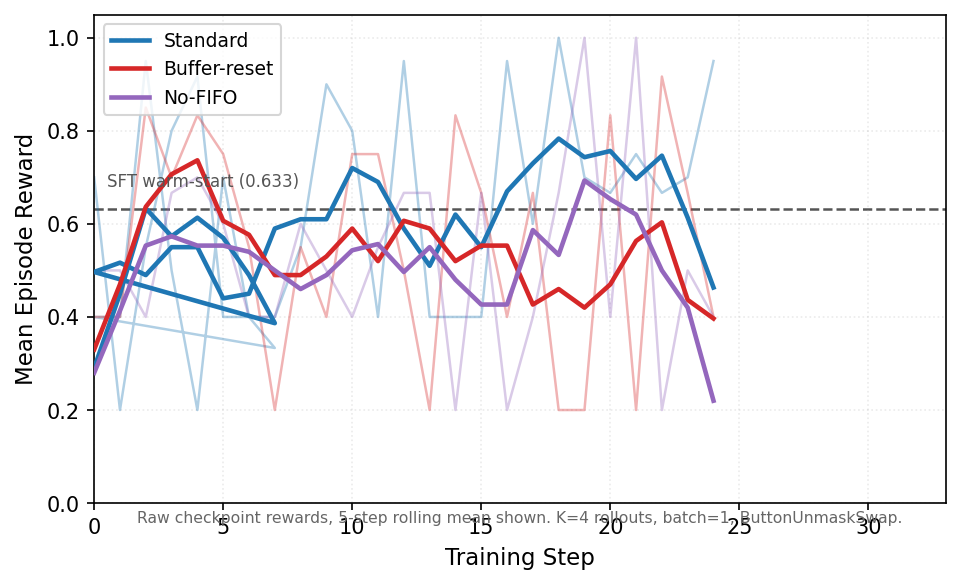
\includegraphics[width=\linewidth]{figures/training_curves.png}
    \end{subfigure}
    \end{center}
    \vspace{0.2em}
    \footnotesize{(a) 5-seed success rates $\pm$ std. (b) Training reward curves, 25 steps (K=4, raw checkpoint values).}

    \vspace{0.4em}
    \textbf{Key finding:} Buffer persistence is \textit{critical} --- clearing the buffer between picks collapses performance to near the memoryless baseline (9.5\% $\approx$ 6.7\%). FIFO context is \textit{expendable} --- no-FIFO (30.7\%) $\approx$ standard (30.0\%). The keyframe buffer carrying pre-occlusion spatial memory across picks is the load-bearing component.

  \end{block}

  \begin{block}{Conclusions \& Future Work}

    \textbf{Result.} Streaming GRPO achieves \textbf{31.4\% $\pm$ 3.1\% SR} on ButtonUnmaskSwap with \textbf{zero human demonstrations}, exceeding MemER-IL (21.3\%, ${\sim}$50 demos/task) by $+$10.1 pp after only 25 training steps.

    \vspace{0.3em}
    \textbf{Engineering lesson.} A coordinate space mismatch between SFT training targets ($\langle y,x\rangle$ 0--256 pixels) and Qwen-VL's native grounding space ($\langle x,y\rangle$ 0--1000) silently caused all RL methods to produce constant subgoal outputs --- zero reward variance, zero gradient. Fixed via \texttt{to\_qwen\_xy}/\texttt{from\_qwen\_xy}. \textit{Diagnostic:} constant predicted coordinates across diverse inputs.

    \vspace{0.3em}
    \textbf{Limitations.} 25 steps $\ll$ convergence (200+ needed); CPU rendering bottleneck (${\sim}$5 min/step); ablation confounded by gradient step count; no binary SR comparison to MemER on the full suite.

    \vspace{0.3em}
    \textbf{Future work.} Longer GRPO runs; GPU-accelerated rollouts; generalization to VideoUnmaskSwap and full Permanence suite; RoboCasa OOD evaluation.

  \end{block}

  \begin{block}{References}
    \tiny
    \nocite{pi05_2024, qwen3vl, grpo_2024, ppo_schulman, robomme, maniskill, memer, mem}
    \bibliographystyle{plain}
    \bibliography{poster}
  \end{block}

\end{column}

\separatorcolumn
\end{columns}
\end{frame}

\end{document}
